\documentclass[tikz,border=10pt]{standalone}
\usepackage{tikz}
\usepackage{tikz-cd}
\usetikzlibrary{arrows,automata,shapes,positioning,decorations.pathmorphing}
% \tikzset{->,>=stealth',auto}
\tikzset{->,auto}
\tikzset{state/.style={shape=circle, draw, fill=white, initial text=,
    inner sep=.5mm, minimum size=2mm}}
\tikzset{state with output/.style={shape=rectangle split, rectangle
    split parts=2, draw, fill=white,
    initial text=, inner sep=1mm}}
\tikzset{every node={font=\footnotesize}}
\begin{document}
  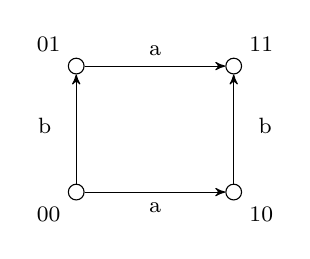
\begin{tikzpicture}[>=stealth', x=1cm, y=.8cm]
    \tikzstyle{every node}=[font=\footnotesize]
    \tikzstyle{every state}=[fill=white,shape=circle,inner
    sep=.5mm,minimum size=3mm]
%    \path[fill=black!15] (0,0) to (2,0) to (2,2) to (0,2) to (0,0);
    \node[state] (00) at (0,0) {};
    \node[state] (10) at (2,0) {};
    \node[state] (01) at (0,2) {};
    \node[state] (11) at (2,2) {};
    \path (00) edge (01);
    \path (00) edge (10);
    \path (01) edge (11);
    \path (10) edge (11);
   % \node at (1,1) {$x$};
    \node at (-.4,1.05) {b};
    \node at (2.4,1.05) {b};
    \node at (1,-.25) {a};
    \node at (1,2.25) {a};
    \node at (-.35,-.35) {00};
    \node at (-.35,2.35) {01};
    \node at (2.35,-.35) {10};
    \node at (2.35,2.35) {11};
  \end{tikzpicture}
\end{document}